\documentclass{article}

\linespread{1.2}
\usepackage[utf8]{inputenc}
\usepackage[left=1.5in,right=1.5in,bottom=1in]{geometry}
\setlength\parindent{0pt}
\setlength{\parskip}{1em}
\setcounter{secnumdepth}{0}
\usepackage{outlines}
\usepackage{graphicx}
\graphicspath{ {imgs} }
\usepackage{hyperref}
\usepackage{color,soul}
\usepackage[normalem]{ulem}

\usepackage[
backend=biber,
style=apa,
citestyle=authoryear,
sorting=nyt,
]{biblatex}
\addbibresource{exam.bib}

\usepackage{comment}
\specialcomment{topicsen}{\begingroup\bfseries\scriptsize}{\endgroup}
%\excludecomment{topicsen}

\newcommand{\alignedmarginpar}[1]{%
        \marginpar{\raggedright\small #1}
    }

\title{Socio-Spatial Urban Diversity}
\author{Carla Hyenne}

\begin{document}

\maketitle

\tableofcontents

\pagebreak

%%%%%%%%%%%%%%%%%%%%%%%%%%%%%%%%%%%%%%%%%%%%%%%%%%%%%%%%%%%%%%%%
%					LECTURE 1
%%%%%%%%%%%%%%%%%%%%%%%%%%%%%%%%%%%%%%%%%%%%%%%%%%%%%%%%%%%%%%%%
\section{Introduction}
\textit{Fieldwork at AAKH}

\subsection{Where do you see diversity?}

Where do you see diversity? Where do you \textbf{not} see diversity? When do socio-spatial effects emerge from ``observed diversity''? Urban diversity in Vienna in comparison to what?

\textit{A photo of a park in Vienna}

There is diversity in the \textbf{built environment} through buildings, public space; in \textbf{functions}, like residential, school, playground, transport; in \textbf{architecture}, through differences in height, density, older vs. modern architecture, balconies and winter gardens, the orientation of the roof (sloped or flat, new builds have flat roofs because they are more affordable to build, increase the potential rent of the top floor, and snow isn't a problem in Vienna anymore); in \textbf{living standards}, social and public vs. private housing; in \textbf{green infrastructure}, trees and grass.

What we do not see are a diversity of people, but could be due to the time of day and year; any \textbf{informal or illegal practices}, meaning anything against pre-defined functional uses, like sleeping rough, graffiti, dancing or performing which could feel unusual; \textbf{ethnic diversity}, there are no restaurants or shops representing minority populations and ethnic communities.

We are asking, \textbf{what is there, or isn't there, and why?}

What processes are causing the diversity, or lack thereof? \textbf{Exclusionary processes}, driven by neoliberal policies and the financialisation of the housing market; 
\textbf{lock-in effects} of the housing market, whereby older social housing buildings and apartments are much more affordable than newly built ones (est. up to twice as less), so even if by European standards rents are still affordable, moving into a newer and smaller (public) apartment can be very expensive. To get social housing, you must have lived in Vienna for some time, thus students and refugees are not eligible;
\textbf{migration} is a global driver of socio-demographic change (both domestic and international), caused by young people moving to the city, in Vienna, a low fertility rate means that migration is necessary to maintain/grow the population. Migration in Vienna is first and foremost domestic, joining the EU in 1995 opened migration to Germany, Eastern Europe, the Balkans, ex-Yugoslavian countries like Serbia Bosnia-Herzegovina, and circa 2015 Syria, Afghanistan, Iraq; 
\textbf{segregation}, which exists in a socially-mixed city like Vienna, even if the `borders' are not so drastic.

\subsection{Super-Diversity}

\textit{```Super-diversity' is proposed as a summary term. Whatever we choose to call it, there is much to be gained by a multidimensional perspective on diversity, both in terms of moving beyond `the ethnic group as either the unit of analysis or sole object of study' (Schiller et al., 2006) and by appreciating the coalescence of factors which condition people's lives''} (Steven Vertovec, 2007)

Ethnic communities are not homogeneous, and ethnicity as a category to speak about diversity is not enough. We require a multidimensional perspective.

\textit{``The basic argument advanced for coining the term and developing the concept is that it describes changing patterns of global migration flows of the post-World War II decades that have entailed the movement of people from more varied national, ethnic linguistic, and religious backgrounds, who occupy more varied legal statuses, and who bring a wide range of human capital (education, work skills, and experience)''} (Foner et al., 2019)

\subsection{Change, everyday life, socio-spatial disparities}

\textbf{Change} what dimensions does ``demographic change'' include in the context of super-diversity?

\textbf{Everyday life} how are practices of living together formed in urban neighbourhoods?

\textbf{Socio-spatial diversity} how do consequences and outcomes manifest in everyday?

Brainstorming \textbf{research questions} based on the reading - use why, what (analytical), how (descriptive)...

\begin{outline}
	\1 Can socio-spatial disparities ever have a positive impact on minority groups? $\rightarrow$ socio-spatial disparities
	\1 When comparing refugees from the Ukrainian war in 2022 and refugees from the Middle-East in 2015 (themselves a highly diverse, non homogenous group), how do public policies and public discourse influence these people's experience and integration into Vienna?
		\2 Change:
		\2 Everyday life:
		\2 Socio-spatial disparities:
\end{outline}


%%%%%%%%%%%%%%%%%%%%%%%%%%%%%%%%%%%%%%%%%%%%%%%%%%%%%%%%%%%%%%%%
%					LECTURE 2
%%%%%%%%%%%%%%%%%%%%%%%%%%%%%%%%%%%%%%%%%%%%%%%%%%%%%%%%%%%%%%%%
\section{Housing Market}

\textit{Guest lecturer Celine Janssen}

\subsection{Housing in Vienna}

A \textbf{housing segment} is a category below housing, which explains the variety of housing types. 

\textbf{Red Vienna} refers to the social policies and the start of communal housing, in the 1920s, when the Social Democrats were in power. This period between the two world wars was particular: Vienna became a province (not only a city) and gained more rights, and could purchase land at an affordable price due to the bad economic situation, which was used for social builds. 
Is `Red Vienna' possible today? No, because in the 1920s the political situation and the land prices were very different to today.

The public (council) housing, or Gemeindebau, are large and imposing buildings. There was a political idea to educate the lower classes, also with culture, and every Gemeindebau must have visible artwork on the outer walls.

Gemeindebau:
\begin{outline}
	\1 Red Vienna Waschsalon
	\1 Gemeindebau in 5th district, on the belt/Gurkel. The idea at the beginning was to provide artists with affordable spaces to do their work, and still today serve this purpose.
\end{outline}

Vienna became the city of affordable housing. This changed with the global financial crisis, after which real estate investment became attractive and subsidised housing was less considered.

\subsubsection{Subsidised rental housing}

There is non-for-profit housing in Vienna, subsidised rental housing which is accessible to those who cannot access council housing. It has public and available open space. 
There are opportunities for public/private partnerships, where private for-profit developers can build housing but must provide affordable rents (cost rent/kostenmiete).

Subsidised rental housing is where new households can move in and find affordable rents, but in the trajectory of social housing, it is the answer to the Gemeindebau whose model would not be efficient today\alignedmarginpar{Why?}.

\subsubsection{Private rental market}

The private rental market is an important sector in Vienna and represents 30\% of the housing. The city has the least influence, or power, in this sector.
The private market is any building built before 1945 (end of WWII) and not owned by the city. Still, the rents are regulated. Rent regulation is a federal law (a national law applying to every Austrian city) and applies to all the private rental houses. The city doesn't have power to change the rent regulation.

New private builds do not fall under rent regulation, and any new builds on top of pre-1945 private housing is also not regulated.

The green party and conservatives who are in power in Austria, find support in private ownership and thus their ideology is not to provide affordable rents. This instead is the ideology of the social democrats. At the city level, with the green and conservative party, you cannot change the rent regulation because you need a majority at the national level. 

To address the private rental market, the city came up with \textbf{soft urban renewal programmes}. It was during a period of time when the city was shrinking, and some old housing stock was decaying and the city was losing buildings due to the lack of financial capacity to renovate. The soft urban renewal programme was the answer, but is often the starting point of the gentrification debate in Vienna.

The private market is highly financialised, they are fully furnished apartments where people/owners do not live full-time but only part of the year, eg. high income expats or investors. This market is unregulated, the price isn't capped and can be sold or rented to the highest bidder.

\subsubsection{Vienna's housing market}

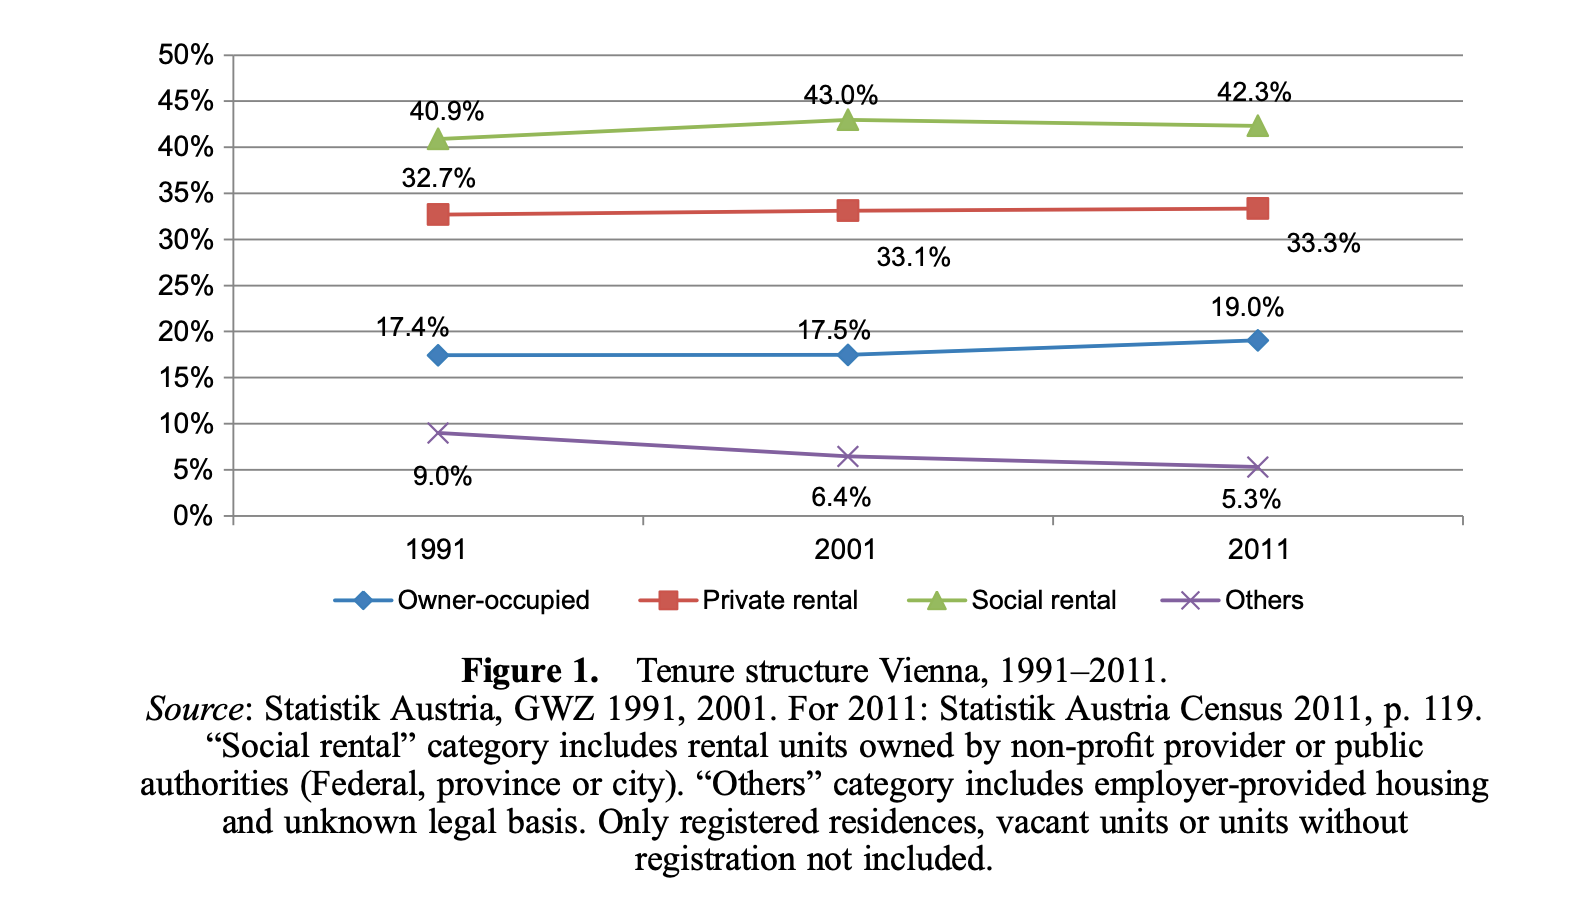
\includegraphics[width=\textwidth]{Vienna_housing_segments}

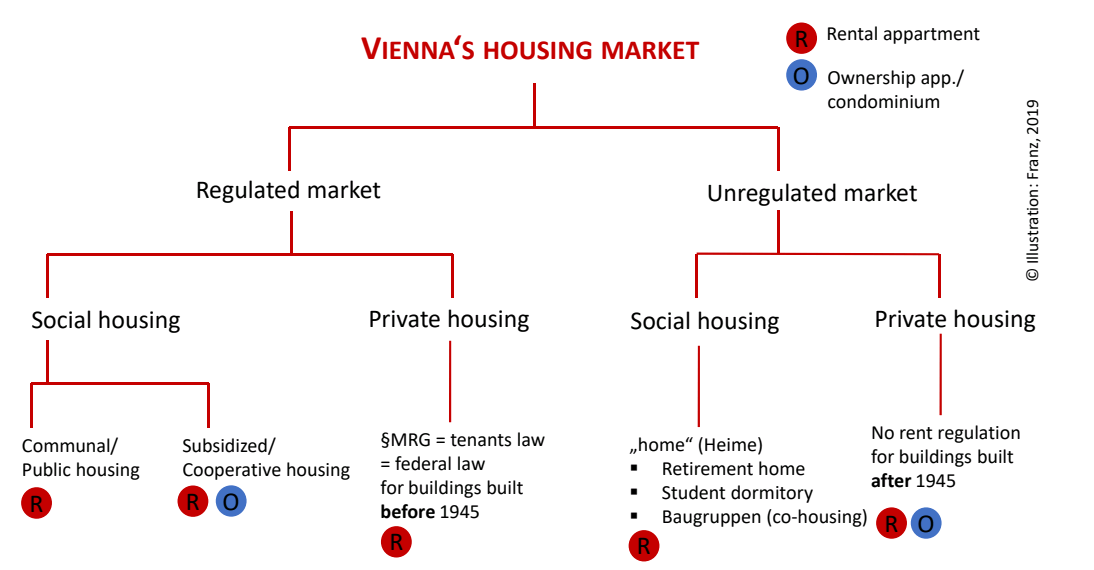
\includegraphics[width=\textwidth]{Vienna_housing_market}

\subsection{Diversity}

How is the housing market related to urban diversity?

Vienna ranks high in the liveable city rankings because of the affordable housing - but the target audience of the rankings, ie. high income expats, will not be the ones to benefit from the affordable or public housing.

\subsubsection{Social mix in a social welfare state}

1230, Vienna: Alterlaa by Harry Glück, in Liesing. Built an alternative mode of living, with high rise buildings but that contain the elements that is important for our standards of living: balconies, private (outdoor) spaces, a swimming pool on the roof, surrounded by open space,  social infrastructure, commercial space (shopping mall) but now more a medical centre, to cater to the aging population in the building.

Social mix, in the UK, was used as an explanation why renovation is taking place, and the effect of renovation is the upgrading of the residential composition. Can this be referred to as State-led gentrification? It created direct displacement, and a buy-out of the apartments.

In the US, property taxes are linked to the value of the property, and a huge interest of the public actor for high property values to get high tax returns. Thus, having a high-income household with low property value results in low tax returns for the city. Social mix is a fiscal policy used to de-concentrate poverty.

The idea is that middle-class households create trickle down effects in their community and are role-models in the lower income households and should participate in social mobility. However, this is incredibly difficult to prove empirically and there is a debate as to whether this is a myth to legitimise gentrification practices.

\subsubsection{From social mix to social mixing}

Social mixing is an effect of daily practices. 
Middle-class households are attracted by ethnically diverse neighbourhoods, but there is no social interactions on a daily basis, and the `social tectonics' are parallel but do not overlap (Jackson and Butler, 2014).

In urban planning, the concept of social mix is used as a political smokescreen without distinct definitions and measures. 

\subsubsection{Planning for social mix }

Seestadt Aspen seems to be ideally planned for social mix.

Who? Actors: public, institutional/individual private, intermediaries. Scales: macro (EU), national, province, city, district neighbourhood.

How? Resources: financial means, time, `power'. Institutional boundaries: laws and regulations.

Why? Rationalities, bounded rationality

\subsection{Who makes the city?}

\textit{Celine Jansenn}

Urban development management focuses on the issues of urban and regional development and institutional design. 

Area development, or regeneration, urban transformation, urban redevelopment projects, are area-based development projects. It focuses on understanding the role of area-based development projects in solving urban problems. 

To research area development, you can take multiple perspectives: spatial, economic, management/corporate, public administration, governance, institutional, etc.

In area development, there are many ideals, but how do you decide what should be developed? There are societal challenges such as CO2 reduction, energy transition, climate adaptation, biodiversity, more affordable housing, alternative mobility, social inclusion, etc. So how do we decide how the land should be used? The design of multifunctional spaces, a political choice.

...

How do you recognise social sustainability in the built environment? There are tangible and intangible ways. Tangible: decent housing, transport, daily facilities, recreation, jobs, schools, public spaces, healthcare, urban design. Intangible: social interaction, social networks, cultural expression, feeling of belonging, feeling of community, safety, wellbeing, existence of informal groups and associations, representation by local governments.


%%%%%%%%%%%%%%%%%%%%%%%%%%%%%%%%%%%%%%%%%%%%%%%%%%%%%%%%%%%%%%%%
%					LECTURE 3
%%%%%%%%%%%%%%%%%%%%%%%%%%%%%%%%%%%%%%%%%%%%%%%%%%%%%%%%%%%%%%%%
\section{Gentrification}

\textit{Fieldwork at XXX}

%%%%%%%%%%%%%%%%%%%%%%%%%%%%%%%%%%%%%%%%%%%%%%%%%%%%%%%%%%%%%%%%
%					LECTURE 4
%%%%%%%%%%%%%%%%%%%%%%%%%%%%%%%%%%%%%%%%%%%%%%%%%%%%%%%%%%%%%%%%
\section{Arrival Space \& the Role of Public Space}

\textit{Fieldwork at XXX}


%%%%%%%%%%%%%%%%%%%%%%%%%%%%%%%%%%%%%%%%%%%%%%%%%%%%%%%%%%%%%%%%
%					LECTURE 5
%%%%%%%%%%%%%%%%%%%%%%%%%%%%%%%%%%%%%%%%%%%%%%%%%%%%%%%%%%%%%%%%
\section{Social Innovation}

\textit{Guest lecturer XXX}


%%%%%%%%%%%%%%%%%%%%%%%%%%%%%%%%%%%%%%%%%%%%%%%%%%%%%%%%%%%%%%%%
%					READINGS
%%%%%%%%%%%%%%%%%%%%%%%%%%%%%%%%%%%%%%%%%%%%%%%%%%%%%%%%%%%%%%%%
\section{Readings}

\subsection{Introduction}

\subsubsection{R. Cavicchia, R, Cucca, \textit{Densification and School Segregation: The Case of Oslo}, 2020}

\begin{outline}
	\1 \textit{tldr;} urban densification is promoted as a desirable thing in cities, making them more sustainable, better social mix, better conditions to live together. However, they can create undesirable residential patterns like segregation and gentrification, and empirical evidence shows that it benefits the richer population. Paper studies residential and specifically school segregation in Oslo, focusing on neoliberal planning approaches
	\1 Why Oslo: growing economically and demographically, has promoted urban densification since the 1980s to prevent urban sprawl, it has an egalitarian social welfare state reflected in the education policies, and school segregation reflects residential segregation because kids are assigned to schools by proximity (`catchment area') > where children live determines where they go to school, thus residential patterns are crucial for understand school segregation in general
	\1 RQ: ``how are the densification developments of the past two decades associated with changes in the distribution of children with different backgrounds in Oslo?''
	\1 Densification policies have to be complemented with policies that counter segregation/gentrification/social inequality that follows
	\1 Oslo
		\2 Strong socio-spatial segregation in Oslo and is considered a `dual-city'. Recent increase in immigration show that immigrants settle in the Eastern, lower income neighbourhoods
		\2 Housing policies shifted since the 1980s, from social to neoliberal, privatised housing markets
		\2 Oslo densification policies are two-fold: from inner to outer city, and along transport lines
	\1 Why does densification lead to segregation?
		\2 
\end{outline}

\subsubsection{Dahinden, Fischer, Menet \textit{Knowledge production, reflexivity, and the use of categories in migration studies: tackling challenges in the field}, 2021}

\begin{outline}
	\1 How are categories, and categorisation, of migrants formulated? And, how can they help reproduce or perpetuate racist and marginalisation discourses? This paper argues we should take a reflexive approach to categories in migration studies
	\1 A turn where terms like society, culture, migration, are revised, and `knowledge production' in migration studies is being given more attention. There is a risk that knowledge production may perpetuate ``particular hegemonic power relations and concomitant forms of social and political exclusion'', ie. reproduce power structures that should no longer exist, and in the worst case, neo-colonial reasoning
	\1 To analyse knowledge production, it uses: the reflexive turn in anthropology and postcolonial scholarship
	\1 Reflexivity is defined here as ``a process of ``decentring'' by distancing one's research from well-established ideas while developing alternative ones'' (p. 536)
		\2 
\end{outline}

\subsubsection{Steven Vertovec, \textit{Talking around super-diversity}, 2019}

\begin{outline}
	\1 \textit{tldr; analyses how different articles or researchers have used and interpreted the term super-diversity, and why the term is widely used}
	\1 The term focuses on migration, and on the ``new social patterns, forms and identities arising from migration-driven diversification'' (abstract). Vertovec believes it has gained popularity because social scientists are looking for ``ways of describing and talking about increasing and intensifying complexities in social dynamics and configurations at the neighbourhood, city, national and global levels'' (p. 135), sometimes through migration patterns, but also through other ``complex social developments''
		\2 It started from the observation in UK migration statistics that migrants came from more countries of origin, thus from a greater diversity of languages, ethnicities, religions... which have created shifts in things like legal statuses, labour market realities, gender and age experiences, residential patterns and segregation, etc. $\rightarrow$ new patterns\alignedmarginpar{change, socio-spatial disparities, everyday life}
		\2 New patterns of inequality, racism, segregation, creolisation (selective blending of cultures)
	\1 Super-diversity has been used in policy circles and by NGO
	\1 A typology of uses of super-diversity 
		\2 as very much diversity
		\2 as a backdrop to a study ie. as a new condition or context, perhaps painting super-diversity as a happy new normal and proving the opposite, and that class and racism still matter
		\2 as more ethnicity, more ethnic groups in a place
		\2 as multidimensional reconfiguration, whereby multiple dimensions need to be taken into consideration when measuring diversity
		\2 as moving beyond ethnicity which is not the optimal unit for analysis, and needing to consider many more aspects in and outside of the ethnic group
		\2 as new or other complexities with regards to migrants, for eg. their place of origin, reasons for migration, careers, sociocultural and linguistic features that can't be assumed; not assuming a direct relation between ethnicity, citizenship, residence, origin, language, profession (p. 132); new social formations, hierarchies, power relations within the migrant group, diverse networks;
	\1 Is super-diversity similar to intersectionality? No, because intersectionality doesn't deal with migration patterns and outcomes, and mostly focuses on race, gender and class
	\1 One limitation in studies and research on ethnicity, are the statistics, data, census collected by States, and the categories they presuppose for people and groups. The studies begin with a set of given categories, rather than looking for better fitting categories
	\1 Change:
	\1 Everyday life:
	\1 Socio-spatial disparities:
\end{outline}

Additional reading: Vershinina, Rodgers, \textit{Symbolic capital within the lived experiences of Eastern European migrants: a gendered perspective}, 2019

\begin{outline}
	\1 How different genders experience migration (transnational, Eastern European) differently, with regards to entrepreneurial activities (eg. opening a business). Through their work, women gain prestige in the eyes of their family and friends back home
	\1 Migrant women: typically depicted as invisible, ``uneducated, illiterate and passive'' (p. 591) but this article explores their agency
	\1 RQ: ``how do transnational migrant entrepreneurs utilise symbolic capital within their entrepreneurial activities in the UK? What role does gender play in this process?''
	\1 Symbolic capital: resources (ie. capital) that is made available to individuals as a result of honour, prestige, recognition
		\2 There is a Soviet concept still present in post-socialist societies (including in Eastern European migrants in the UK) where one uses their personal connections to get ahead, and another concept where people identify others as `one of us' and form communities
\end{outline}

\subsection{Gentrification}

\subsubsection{Lees, \textit{A reappraisal of gentrification: towards a `geography of gentrification'}, 2000} \parencite{lees2000reappraisal}

\begin{outline}
	\1 $\rightarrow$ What does gentrification mean in general with regard to processes and effects?
	\1 Focus points for research on the geography of gentrification: ``1) financifiers - super-gentrification; 2) third-world immigration - the global city; 3) black/ethnic minority gentrification - race and gentrification; 4) liveability/urban policy - discourse on gentrification''
	\1 Gentrification is creating conflict between working class and yuppies/middle-upper classes (p. 390). This is happening not only in global cities, and follows political and economic phenomenons (fall of iron curtain created gentrification in eastern Europe, eg. Prague)
	\1 1990s gentrification literature focused on urban policy and urban politics. Governments mixed ``urban regeneration policy with gentrification practices and environmentalism'' (p. 391). Gentrification is being used for liveability and environmental sustainability
	\1 Rebranding of gentrification by politicians as promoting urban renaissance, to support a `move back to the city' in Britain, for eg.
	\1 Other important issues linked to gentrification: race and financification (p. 392)
	\1 The emancipatory city
		\2 Lefebvrian, ``space is produced and reproduced as a site of social, political and economic struggle'' (p. 393); 
		\2 Emancipation is inscribed in gentrification, in the agency of the gentrifiers; gentrification as an emancipatory social practice; gentrifiers as a diverse group of people, creating tolerance
			\3 Some positions, cultural practices and class factions are privileged over others
		\2 But is there really a link between living in the old inner city, and tolerance? Do exchanges between people make them tolerant, or are interactions in the city disinterested?
			\3 There are divergent interests, between the gentrifiers and the anti-gentrification groups/working class/ethnic minorities; even if they live next to each other, what they want from their space and their neighbourhood differs
			\3 Often, the interests of gentrifiers win over others because they are able to, and want to, pay more; they have more economic, cultural and social resources (p. 394)
		\2 Gender and gentrification: gentrification was linked to marginal groups, and patriarchal emancipation brought in gender dimension; similar to gays
	\1 The new middle class
		\2 Synonymous to the emancipated gentrifier, using the inner city as a place of emancipation, is less conservative than the old middle class; from hippies to yuppies, gentrifiers is a post-industrial society
		\2 A difference in gentrifiers, eg. between Hackney and the Docklands, where one gentrified neighbourhood is the result of a community choice and formation, and the other the logic of capital. 
		\2 Financifiers and regentrifiers: those moving in to already gentrified neighbourhoods, and buying the property of the original gentrifiers; are they really gentrifiers, if that are not displacing marginalised populations? (p. 398)
	\1 The revanchist city
		\2 Revenge against the poor and minorities who stole the inner city from the upper ``respectable'' classes (p. 399); urban regeneration, gentrification, disguises the violence of the process; a retaking of the city
		\2 The silent displacement of minority communities (Black, Bengali...) by white communities/gentrifiers\
	\1 At the time this paper was written, class and gender research on gentrification outweighed ethnic and racial research
\end{outline}

\subsubsection{Gruber, \textit{What Can the Housing Market Teach Us? University Fieldtrips Identify Current Transitions in Vienna's Urban Development and Housing Market Policies}} \parencite{gruber2020can}

\begin{outline}
	\1 $\rightarrow$ How does local housing market transition in Vienna relate to gentrification
	\1 Vienna is famous for its social housing, due in part to Red Vienna and the Soft Urban Renewal Programme
	\1 Large number of public housing, but an increasing rent and cost of housing shows the increasing demand, as so the increase in housing buildings, both public and private
	\1 Reasons for contemporary issues on housing: ``general transformation processes such as population growth, new migration patterns, global financial investment practices and (ostensibly) limited resources for ensuring a supply of affordable housing'' (p. 382)
	\1 Red Vienna and social democrats
		\2 In power 1919-1934, main goal was to raise quality of life for workers, which included extensive social housing policies. Also introduced a housing tax, which made it possible to finance new buildings (Gemeindebauten). Many of the Gemeindebauten were built after WWII, and a revival programme started in the 2000s to create 120 flats for use by 2019
		\2 Prior to Gemeindebauten, housing was driven by private market and speculation
	\1 Gemeindebauten
		\2 Specific requirements to fulfil in order to qualify for a flat 
	\1 Population dynamics: at the end of 20th century, it was the suburbs that were growing, but since mid-2000s, the inner city is growing again, especially due to migration from the EU and since mid-2010s, from middle east/asylum seekers
	\1 Challenges
		\2 2008 financial crisis resulted in increase interest from private investors in real estate market, and has driven most of the gentrification and put pressure into de-commodifying the social housing market
		\2 Countering investors and the rise in housing costs, with the European Citizen Petition ``Housing for All'' (2019)
		\2 Private investors have been sought out to renovate the old housing stock that the city does not have the money to maintain, and also to keep up with the growing demand
	\1 Strategies for affordable housing
		\2 Competition for for-profit and non-profit developments on the available plots of the New Leopoldau (21st district)
		\2 New zoning to accommodate more public-supported housing 
		\2 Policies to protect old housing stock from the founders period
		\2 The ``soft urban renewal programme'' in the 1970s was a special subsidy for private building owners to do renovations, but with minimal increase in rental prices
\end{outline}

\section{Assignments}

\pagebreak

\begin{flushright}
Carla Hyenne 12138698\\
Socio-Spatial Urban Diversity SS2022
\end{flushright}

\textit{Formulate three hypotheses on the local context of Vienna with regard to gentrification, and include 1-3 signifiers you might search for in the built environment to support or to object the hypothesis.}

\textbf{Hypothesis}: Vienna actively employs social mix policies to counter (or justify?) gentrification.\\
\textbf{Signifiers}: presence of public and private housing, and their proximity to one another; presence of ethnic shops and services; a diversity of users, in age, income, culture, ethnicity...;

\textbf{Hypothesis}: in contrast to the era of Red Vienna, today's (conservative) government has created an atmosphere in which tensions between social classes are rising. \\
\textbf{Signifiers}: signs of protests against gentrification phenomenons like urban regeneration project, real estate developments, increased unaffordability of housing (banners, posters, stickers); signs of private real estate developers/private housing projects (advertisement, building permits, building sites); informal and illegal behaviours like squats, rough sleeping, graffiti;

\textbf{Hypothesis}: gentrification is being caused by the ``soft urban renewal'' programme, where old public housing stocks are renovated by private real estate investors and developers. \\
\textbf{Signifiers}: renovation projects of old public housing by private developers; the number of private dwellings near the renovations;

\begin{comment}

\textbf{Hypothesis}: due to the social and subsidised housing context in Vienna, gentrification has been limited because the new middle class did not displace marginal groups \\
\textbf{Signifiers}: evolution of the geography of household income; evolution of demand for social and subsidised housing; evolution of social housing provision;

\textbf{Hypothesis}: Gentrification in Vienna is limited due to the geography of the social and subsidised housing
\textbf{Signifiers}: location of social and subsidised housing; rent and property price trends; trends of private ownership of housing;

\textbf{Hypothesis}: Liveability, environmental sustainability, a ``civilised life'' \parencite{lees2000reappraisal} cannot be achieved without gentrification / or, can be achieved in Vienna without gentrification, 
\textbf{Signifiers}: political discourse on liveability/urban regeneration

\textbf{Hypothesis}: gentrification in Vienna has an ethnic or racial dimension.
\textbf{Signifiers}: what ethnicities are represented in the shops and services, and which aren't;  
ethnicities of those living in social and subsidised housing; ethnicities of those living in private housing; ???;

\textbf{Hypothesis}: the social housing and welfare system in Vienna has allowed working classes, or their children, to move up the social scale and become gentrifiers
\textbf{Signifiers}: housing patterns of children with working class parents; ???; ???; 

\textbf{Hypothesis}: due to its social policies, including the availability of social and subsidised housing, Vienna has kept the gap between the working and middle class fairly small
\textbf{Signifiers}: wealth gap between population living in public housing vs. private housing; ???; ???;

\textbf{Hypothesis}: the conservative national government and the local government created a friendlier environment for private real estate investors, who are rising rent and property prices in once-affordable neighbourhoods\\
\textbf{Signifiers}: rent and property prices trend; number of private investors and developers; ???;

\textbf{Hypothesis}: the amount of social housing in Vienna allows the lower class to have a relatively high quality of life. This reduces, or even prevents, conflicts between social classes and the marginalisation of vulnerable populations. \\
\textbf{Signifiers}: no signs of protests/signs of enthusiasm towards regeneration projects, private investments and developments; social housing complex and populations are integrated into the urban fabric, not excluded; 

\textbf{Hypothesis}:
\textbf{Signifiers}:


\end{comment}

\pagebreak

\end{document}


%%%%%%%%%
\begin{comment}

\subsubsection{\textit{}}

\begin{outline}

\end{outline}

\end{comment}

